% Chapter Chapter 4 For Reproducible Research in R and RStudio
% Christopher Gandrud
% Created: 16/07/2012 05:45:03 pm CEST
% Updated: 21 September 2012




\chapter{Getting Started with File Management}\label{DirectoriesChapter}

Careful file management is crucial for reproducible research. Apart from the fleeting situations where you have am email exchange (or even meet in person) someone interested in reproducing your research, the main information other researchers will have is stored across many files: data files, analysis files, and presentation files. If these files are well organized then replication will be easier. File management is also important for you as a researcher, because if your files are well organized you will be able to understand your work more easily. Remember two of the guidelines from Chapter \ref{GettingStartedRR}:

\begin{itemize}
    \item Reproducible research projects are many files explicitly tied together,
    \item Have a plan to organize, store, and make your files available. 
\end{itemize}

Using tools such as R and markup languages like \LaTeX requires a bit more knowledge of how files are located--their {\bf{path}}\index{file path}--in your computer and on the internet than just knowing which graphical folder they are located in. Though more difficult to use at first than the typical point-and-click graphical user interface file handling systems you are probably familiar, R and Unix-like shell programs allow us to control files--creating, deleting, moving them--in powerful and reproducible ways. 

In this chapter we discuss how a reproducible research project may be organized and cover the basics of file path naming conventions\index{file path naming conventions} in Unix, Mac, and Windows systems. We then learn how to navigate through files in RStudio in the {\bf{Files}} pane as well as some basic R and Unix-like shell commands for manipulating files. The skills we learn in this chapter will be heavily used in the next Chapter (Gathering Data with R) and throughout the book.

In this chapter we work with locally stored files\index{locally stored}, i.e. files stored on your computer. In the next chapter (Chapter \ref{Storing}) we will discuss various ways to store and access files stored remotely in the cloud\index{cloud storage}.

\section{Organizing your research project}

Figure \ref{ExampleTree} gives an example of how the files in a simple reproducible research project could be structured. The project--called {\emph{Example Project}}--is organized into three main parts: a data gathering section, an analysis section, and a presentation section. The results of the project are presented in an article, slideshow, and website.

COMPLETE

The \textt{README.md} file\index{README file} should briefly describe the project including things such as its title, author(s), and so on. It should also indicate how the folders in the project are organized and how to reproduce the project. This will likely include information on the directory names that you used. The README file should be in the main project folder so that it is easy to find. If you are storing your project as a GitHub\index{GitHub} repository (see Chapter \ref{Storing}) and the file is called \texttt{README} its contents will automatically be displayed on the repository's main page. If it is written using Markdown, it will also be properly formatted.

It is good practice to dynamically include the system information for the R session you used to create the project. To do this you can write your readme file with R Markdown. Simply include the \texttt{sessionInfo()} command in a code chunk in the R Markdown document. If you knit this file immediately after knitting your presentation document it will record the information for that session.

%% Make file discussion?

\clearpage
\thispagestyle{plain}
\begin{landscape}
\begin{figure}[th!]
    \caption{Example Research Project File Tree}
    \label{ExampleTree}
    \begin{center}
    
    \documentclass{article}

\usepackage{tikz}

\begin{document}

%%%%%% Example 

\tikzstyle{DirBox} = [draw=black, rectangle, minimum width=5em, thick]
  
\begin{tikzpicture}
  % Root Directory
  \node (root) at (5, 10) [DirBox]{Root};
  
  % Project Directory
  \node (project) at (5, 8.5) [DirBox]{Project};
  
  % Main Project sub-directories
  \node (data) at (2, 7) [DirBox]{Data};
  \node (analysis) at (5, 7) [DirBox]{Analysis};
  \node (presentation) at (8, 7) [DirBox]{Presentation};
  
  % Data subdirectories/files
  \node (dataGatherSource) at (-0.5, 6) [DirBox]{GatherSource};  
  \node (dataFiles) at (2, 6) [DirBox]{DataFiles};
  
  \node (dataMake) at (-0.5, 5.25) {{\small{DataMakeFile.R}}};
  
  \node(dataGather) at (-0.5, 4.5) [DirBox]{IndvDataGather};
  \node (dataGather1) at (-0.5, 3.5) {{\small{DataGather1.R}}};
  
  % Analysis subdirectores/files
  
  % Presentation subdirectories/files
  
  % Connect boxes
  \draw (root) -- (project);
  \draw (project) -| (data);
  \draw (project) -- (analysis);
  \draw (project) -| (presentation);
  
  %% Data connect boxes
  \draw (data) -| (dataGatherSource);
  \draw (data) -- (dataFiles);
  \draw (dataGatherSource) -- (dataMake);
  
\end{tikzpicture}



\end{document}
    \end{center}
\end{figure}
\end{landscape}

\section{File paths \& naming conventions}

All of the operating systems\index{operating systems} covered in this book use organize files in in hierarchical directories\index{directories} (or file trees). To a large extent, `directories' can be thought of as the folders you usually see on your Windows or Mac desktop. They are called `hierarchical' because directories are located inside of other directories, like we saw in Figure \ref{ExampleTree}. 

\subsection{Root directories}

A root directory is the highest directory level in a disk, such as a hard drive.

\subsection{Working directories}

\section{Operating system-specific naming conventions}

\paragraph{Unix}

\paragraph{Mac}

\paragraph{Windows}

\section{File navigation in RStudio}

The RStudio {\bf{Files}} pane allows us to navigate and do some basic file manipulations. Figure \ref{FilesPane} shows us what this pane looks like.

\begin{figure}[t!]
    \caption{The RStudio Files Pane} %\\[0.25cm]
    \label{FilesPane}
        \begin{center}    
        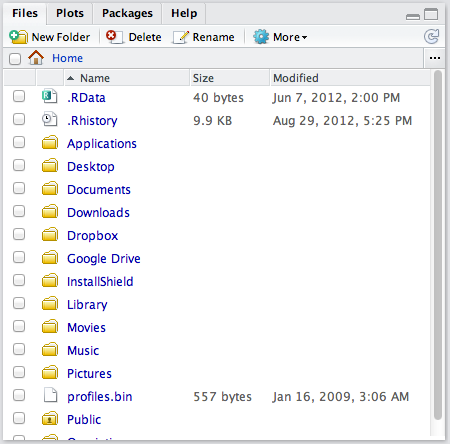
\includegraphics[scale=0.4]{/git_repositories/Rep-Res-Book/Source/Children/Chapter4/images4/RStudioFiles.png}
        \end{center}
\end{figure}

\section{R file manipulation commands}

All of the tasks we can accomplish in RStudio's {\bf{Files}} pane can also be accomplished using command line R. This allows us to more easily replicate our actions. 

\paragraph{{\tt{setwd}}}

The {\tt{setwd}} command sets the working directory.

\paragraph{{\tt{dir.create}}}

Sometimes we may want to create a new directory. We can use the {\tt{dir.create}} command to do this.

\paragraph{{\tt{unlink}}}

You can use the {\tt{unlink}} command to delete a file, files, or directories. 

\section{Unix-like shell commands} 

Though this book is mostly focused on using R for reproducible research it can be useful to use a Unix-like shell program to manipulate files in large projects. A command line shell program is simply a program that allows you to type commands to interact with your computer's operating system.\cite{ShottsJr2012} We will especially return to shell commands near the end of the book when we discuss Make files\index{Make files} for compiling large documents, and batch reports\index{batch reports} (Chapter \ref{LargeDocs}). The syntax discussed here is also similar to the used in command line git (Chapter \ref{Storing}) and Pandoc (Chapter \ref{LargeDocs}). We don't have enough space to properly get started with shell programs. For good introductions for Unix and Mac OS 10 computers see William E. Shotts Jr.'s book on the Linux command-line\cite{ShottsJr2012} and for Windows users Microsoft maintains a tutorial on Windows PowerShell at \url{http://technet.microsoft.com/en-us/library/hh848793}.

The one piece of general instruction I will give now is to highlight an important difference in the syntax between R and shell commands. In shell commands you don't need to put parentheses around your arguments. For example if we want to change our working directory to my Mac Desktop in a shell using the {\tt{cd}} command we simply type:

\begin{knitrout}
\definecolor{shadecolor}{rgb}{0.969, 0.969, 0.969}\color{fgcolor}\begin{kframe}
\begin{verbatim}
cd ~/Desktop
\end{verbatim}
\end{kframe}
\end{knitrout}


\paragraph{{\tt{cd}}}

As we just saw, to change the working directory in the shell can just use the {\tt{cd}}\index{cd} (change directory) command.

\paragraph{{\tt{rm}}}

The {\tt{rm}}\index{rm} command is similar to R's {\tt{unlink}} command. It deletes files or directories.
